\section{Processing Setup }\label{sec:methods}
\interfootnotelinepenalty=10000
We will study two types of parameters in our scalability model. The first parameter type is the  


\subsection{Processing metrics}
Mention the pipeline steps influxdb and telegraf and how telegraf records the current pipeline step. Discuss the importance of only tracking programs running in the current session (shared nodes) and the modification to telegraf to do this (subsection)
Discuss all the metrics collected automatically by telegraf and the tagging in inlfuxdb. 



%\begin{figure}
%    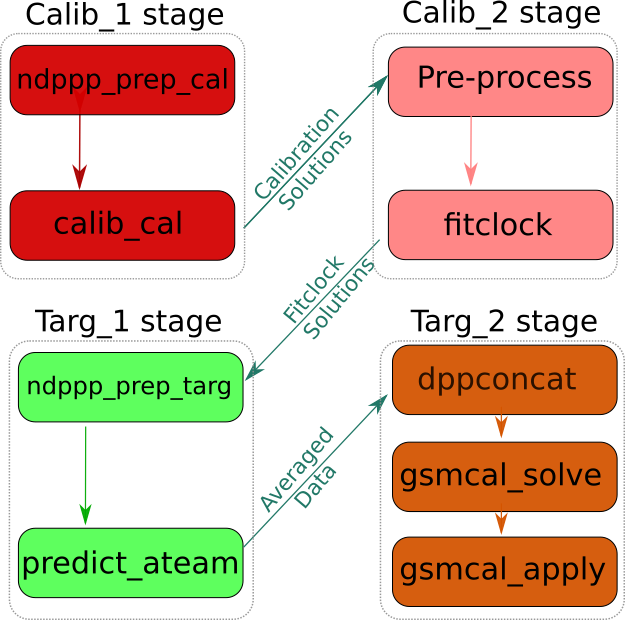
\includegraphics[width=0.95\linewidth]{figures/4_stages_steps1.png}
%      \caption{The four processing stages that make up the prefactor pipeline. The Calibrator %stages (top) process a known bright calibrator to obtain the gain for the LOFAR antennas. The %Target stages (bottom) process the scientific observation to remove Direction Independent %effects.}
%	\label{fig:four_steps_box}
%\end{figure}

\subsection{Non-software performance}
Staging files at different locations can be modelled using historical data, discuss the importance of knowing the time it takes to stage data and the prediction of future performance. 
Queueing jobs can take significant amount of time compared to processing, discuss importance of choosing the optimal processing parameters to optimize the queueing/processing time for each job. 

\subsubsection{Software versions}\label{sec:software_versions}
Maybe talk about singularity and software distribution (and how it's kept constant)

\subsection{Test Hardware}
Short discussion of the different hardware that we run on as part of the queueing system. 
